%
% VorlagePraxisbericht.tex		
% 	
% Florian Kalinke
% 09.09.2013
%				
% Daniel Betsche	
% 05.09.2014 					

\documentclass[pdftex,12pt,a4paper]{article}

\usepackage[utf8]{inputenc}
\usepackage[ngerman]{babel}
\usepackage[T1]{fontenc}
\usepackage[pdftex]{graphicx}
\usepackage{float}
\usepackage{tabularx}
\usepackage{multirow}
\usepackage[hyphens]{url}
\usepackage{geometry}
\geometry{a4paper,left=25mm,right=25mm, top=1cm, bottom=25mm, includeheadfoot}
\usepackage{fancyhdr}
\usepackage{setspace}
\usepackage[usenames, dvipsnames]{color}
\usepackage{listings}	% for code
\usepackage{xcolor}
%\usepackage{hyperref}  % auskommentieren um verlinkungen zu ermöglichen
\lstset{language=Java}

\onehalfspacing	% Zeilenabstand erhöhen

% Kopf- und Fußzeilen einbinden
\pagestyle{fancy}
\fancyhf{}
\fancyhead[R]{Seite \thepage}
\renewcommand{\headrulewidth}{0.5pt}

% Schriftart auf Arial setzen
\renewcommand{\rmdefault}{phv} % Arial
\renewcommand{\sfdefault}{phv} % Arial

\begin{document}
% Um Java Code einzubinden
\definecolor{javared}{rgb}{0.6,0,0} % for strings
\definecolor{javagreen}{rgb}{0.25,0.5,0.35} % comments
\definecolor{javapurple}{rgb}{0.5,0,0.35} % keywords
\definecolor{javadocblue}{rgb}{0.25,0.35,0.75} % javadoc

% Um XML Code einzubinden
\definecolor{gray}{rgb}{0.4,0.4,0.4}
\definecolor{darkblue}{rgb}{0.0,0.0,0.6}
\definecolor{cyan}{rgb}{0.0,0.6,0.6}

% Die lstlisting style Definitionen
\colorlet{punct}{red!60!black}
\definecolor{background}{HTML}{EEEEEE}
\definecolor{delim}{RGB}{20,105,176}
\colorlet{numb}{magenta!60!black}

% http://tex.stackexchange.com/questions/10255/xml-syntax-highlighting
\lstset{
	basicstyle=\ttfamily,
	columns=fullflexible,
	showstringspaces=false,
	commentstyle=\color{gray}\upshape
}
\lstdefinelanguage{XML}
{
	basicstyle=\normalfont\ttfamily\bfseries,
	morestring=[b]",
	morestring=[s]{>}{<},
	morecomment=[s]{<?}{?>},
	stringstyle=\color{black},
	identifierstyle=\color{delim},
	keywordstyle=\color{delim},
	breaklines=true,
  frame=lines,
  backgroundcolor=\color{background},
	morekeywords={
		xmlns,version,type,properties,key,name,description,type,values,property
	}% list your attributes here
}
% http://texblog.org/2011/06/11/latex-syntax-highlighting-examples/
\lstdefinestyle{customjava}{
	language=Java,
	basicstyle=\normalfont\ttfamily,
	keywordstyle=\color{javapurple}\bfseries,
	stringstyle=\color{javared},
	commentstyle=\color{javagreen},
	morecomment=[s][\color{javadocblue}]{/**}{*/},
	numbers=none,
	stepnumber=2,
	numbersep=10pt,
	frame=lines,
	backgroundcolor=\color{background},
	tabsize=4,
	showspaces=false,
	showstringspaces=false
}
% http://tex.stackexchange.com/questions/83085/how-to-improve-listings-display-of-json-files
\lstdefinelanguage{json}{
    basicstyle=\normalfont\ttfamily,
    numbers=none,
    numberstyle=\scriptsize,
    stepnumber=1,
    numbersep=10pt,
    showstringspaces=false,
    breaklines=true,
    frame=lines,
    backgroundcolor=\color{background},
    literate=
     *{0}{{{\color{numb}0}}}{1}
      {1}{{{\color{numb}1}}}{1}
      {2}{{{\color{numb}2}}}{1}
      {3}{{{\color{numb}3}}}{1}
      {4}{{{\color{numb}4}}}{1}
      {5}{{{\color{numb}5}}}{1}
      {6}{{{\color{numb}6}}}{1}
      {7}{{{\color{numb}7}}}{1}
      {8}{{{\color{numb}8}}}{1}
      {9}{{{\color{numb}9}}}{1}
      {:}{{{\color{punct}{:}}}}{1}
      {,}{{{\color{punct}{,}}}}{1}
      {\{}{{{\color{delim}{\{}}}}{1}
      {\}}{{{\color{delim}{\}}}}}{1}
      {[}{{{\color{delim}{[}}}}{1}
      {]}{{{\color{delim}{]}}}}{1},
}
 %Stil des Dokuments festlegen

\pagenumbering{Roman}

\begin{titlepage}
	\begin{center}
		\begin{minipage}{0.4\textwidth}
			\begin{flushleft}
				
\includegraphics[scale=0.9]{./logos/DHBW}
			\end{flushleft}
		\end{minipage}
		\begin{minipage}{0.4\textwidth}
			\begin{flushright}
				%
\includegraphics[scale=0.6]{./logos/Fiducia}
			\end{flushright}
		\end{minipage}
		\\[1.5cm]
		{\LARGE Social Funnel - Software Requirements Specification}\\[1.5cm]

		\textsc{\Large Vorlesung Wintersemester 2014}\\[0.5cm]

		3. Semester\\[1.5cm]
		des Studiengangs Angewandte Informatik\\
		an der\\
		Dualen Hochschule Baden-Württemberg Karlsruhe\\[1.5cm]
		von\\
		Laura Ichters, Simon Brückl, Daniel Betsche\\

		\vfill

		\begin{tabular}{l l}
			Vorlesungszeitraum	& 29.09.2014 - 22.12.2014 \\
			Kurs			& TINF13B2 \\
			Dozent		& Kay Magarethe Berkling
		\end{tabular}
	\end{center}
\end{titlepage}
	% Deckblatt

\newpage
\tableofcontents
\newpage
%\listoffigures %Bildverzeichnis
%\newpage
\pagenumbering{arabic}

%content

\section{Introduction}

Dieser Abschnitt gibt eine Übersicht über die Idee von ``Social Funnel'', sowie seine Funktionen und 
der allgemeine Sinn der Anwendung.

\subsection{Purpose}

Der Sinn dieses Dokuments ist es, eine detaillierte Beschreibung der Anforderungen für “SocialFunnel'' zu definieren.
Es enthält alle notwendigen Informationen für die Entwicklung dieser Anwendung sowie alle Angaben zu
seinem Verwendungszweck. Hier werden alle Einschränkungen, Schnittstellen und Wechselwirkungen mit
externen Plattformen beschrieben und erklärt. Die primäre Absicht des Dokuments ist es, eine Übersicht
für Entwickler zu geben und eine Richtlinie für den Entwicklungsprozess darzustellen.

\subsection{Scope}

“Social Funnel” ist eine Webanwendung, basierend auf bekannten und bewährten Sozialen Medien. Die
Idee ist, dass die schiere Menge an Informationen aus Sozialen Medien nicht mehr überschaubar ist.
“Social Funnel” zielt darauf ab, dieses Chaos zu bereinigen und eine einfache und nützliche Übersicht für
neue Nachrichten, Ereignisse und Posts zu schaffen. Die unterstützen Platformen werden dabei in einen 
einzigen Nachrichtenfeed zusammengeführt und dieser mit verbesserten Werkzeugen für das
Sortieren und Filtern ausgestattet.\\
 
 Für eine einfachere Kommunikation und die Eliminierung von Wiederholung bietet “Social Funnel” ein
 Eingabe-Formular an, mit dem sich auf allen angebundenen und unterstützen Sozialen Netzwerken gleichzeitig
 ein neuer Post verfassen lässt. Anstatt also auf jeder Plattform einzeln seine Neuigkeiten zu verbreiten
 kann dies alles mit einem einzigen Beitrag geschehen. Diese Technologie erspart nicht nur zeit, sonder 
 reduziert gleichzeitig mögliche Fehlerquellen und erhöht die Übersichtlichkeit.\\
 
 Die Software selbst benötigt einen modernen Browser, welcher fähig ist JavaScript auszuführen, sowie eine
 aktive Internetverbindung. Außerdem ist für den Gebrauch der Software mindestens ein Account auf 
 einem unterstützen sozialen Netzwerk notwendig, allerdings nicht für die Registrierung bei “Social Funnel”.
 Die Accounts können einfach miteinander verbunden werden oder aus der Anwendung heraus
 erstellt.

\subsection{Definitions, Acronyms and Abbreviations}

\begin{center}
%\newline \begin{tiny}
%Quelle: Neutrino Mass ISSN 0081-3869
%\end{tiny}
\begin{tabular}[h]{|c|c|}
  \hline
  Begriff   & Definition \\\hline
  User   & Person mit Internet-Anschluss und Accounts in einem oder \\ 
            & mehreren Sozialen Netzwerken\\\hline
  Admin & Person die User-Aktionen überwacht \\ 
  	  & und aufkommende Probleme löst \\\hline
  Entwickler & Person die das Programm entwickelt und Funktionen implementiert\\\hline
  Soziale Medien & Software die Menschen miteinander verbindet\\\hline
\end{tabular}
\end{center}

\subsection{References}

% Die bibliographie eben, alles quellenangaben
%\bibliographystyle{plain}
%\bibliography{bib}
To be determined

\subsection{Overview}

Das Dokument enthält ab dieser Stelle drei Kapitel und Anhänge. Das Zweite Kapitel beinhaltet eine
Übersicht der Funktionen der Anwending, des Designs und den Interaktionen mit externen Plattformen.
Weiterhin definiert und beschreibt das Kapitel die Einschränkungen des Systems.\\

Das dritte Kapitel liefert die Requirements Specification in detaillierten Bedingungen und eine 
Beschreibung der verschiedenen genutzten Schnittstellen.\\

Das vierte Kapitel diskutiert unterstützenden Informationen über das Projekt und die angebundenen
externen Platformen welche darin genutzt werden.

\section{Overall Description}

Dieser Bereich behandelt eine Übersicht der Anwendung als Ganzes. Hier beschreiben wir sie in ihrem
Kontext and der vollen Breite ihres Designs, Arbeitsabläufe und Funktionen. Außerdem definieren wir eine
Zielgruppe und genaue Instruktionen wie der erwartete Verwendungszweck der Anwendung.

\subsection{Use-Case Model Survey}

\begin{center}
	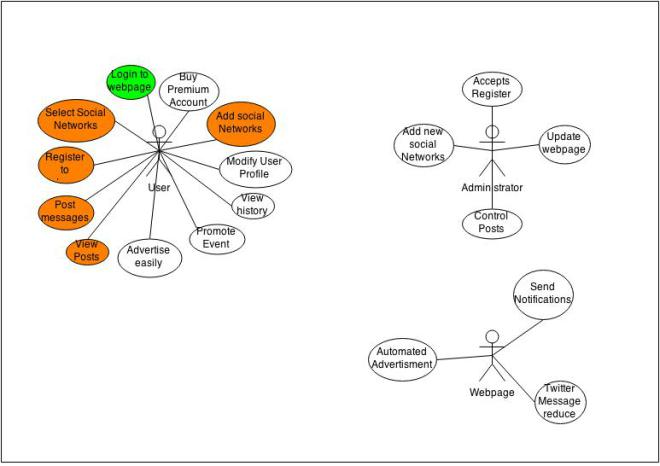
\includegraphics[width=16cm]{./img/usecase_socialfunnel.jpg}
\end{center}
	
To be determined
 
\subsection{Assumptions and Dependencies}

\paragraph{Vorraussetzungen:} Für den gebrauch der Anwendung braucht der Nutzer einen Internetzugang, 
sowie einen Account bei einem der Sozialen Netzwerke, die eingebunden werden.
Auch muss er sich innerhalb der Webanwendung einmal in den gewünschten sozialen Netzwerken anmelden, 
um diese über den Account der Web-Anwendung nutzen zu können.\\

\paragraph{Abhängigkeiten:} Die Anwendung funktioniert nur, wenn die Zielsysteme (Sozialen Netzwerke) funktionieren. 
Sollte es auf einer der anderen Seiten Probleme geben, kann diese nicht angesprochen werden.\\

\section{Specific Requirements}

To be determined

\subsection{Use-Case Reports}

To be determined

\subsection{Supplementary Requirements}

To be determined

\section{Supporting Information}

To be determined

\end{document}